\documentclass{standalone}
\usepackage{tikz}

\begin{document}

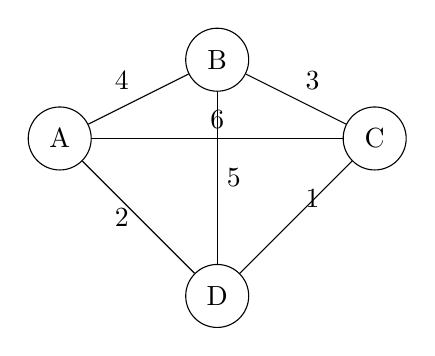
\begin{tikzpicture}[scale=1, transform shape]
    % Nodos
    \node[circle, draw, minimum size=0.8cm] (A) at (0,0) {A};
    \node[circle, draw, minimum size=0.8cm] (B) at (2,1) {B};
    \node[circle, draw, minimum size=0.8cm] (C) at (4,0) {C};
    \node[circle, draw, minimum size=0.8cm] (D) at (2,-2) {D};
    % Aristas con pesos
    \draw (A) -- node[midway, above left] {4} (B);
    \draw (B) -- node[midway, above right] {3} (C);
    \draw (A) -- node[midway, left] {2} (D);
    \draw (B) -- node[midway, right] {5} (D);
    \draw (C) -- node[midway, above right] {1} (D);
    \draw (A) -- node[midway, above] {6} (C);
\end{tikzpicture}

\end{document}
